Ce projet a pour but de développer un modèle permettant de catégoriser des emails en spam ou ham.
La définition d'un spam dans le dictionnaire \emph{Larousse} est :

\begin{quote}
	Courrier électronique non sollicité envoyé en grand nombre à des boîtes aux lettres électroniques ou à des forums, dans un but publicitaire ou commercial.
\end{quote}

Il est possible d'ajouter à cette catégorie tous les mails indésirables comme les tentatives d'hameçonnage permettant de soutirer des informations personnelles à une cible.\\ 

L'objectif est de travailler uniquement sur les données textuelles issues du corps du mail.
Nous avons donc comme point de départ les éléments suivants :
\begin{itemize}
	\item langue : anglais
	\item corpus : monolingue écrit
	\item type : e-mail
\end{itemize}

\paragraph{Déroulé} Le développement de ce projet s'articule autour de 3 phases majeures
	\begin{itemize}
		\item Phase 1 : Récupération des données (Fouille de données)
		\item Phase 2 : Analyse des caractéristiques (Traitement de langage)
		\item Phase 3 : Construction d'un modèle d'analyse (IA)
	\end{itemize}


\subparagraph{Phase 1} La phase 1 concerne la récolte des informations et les traitements minimums nécessaires pour la mise en base.
Les objectifs de traitement de cette phase sont :
\begin{itemize}
	\item Extraire les corps des mails et éliminer les méta-données superflues
	\item Éliminer les mails non anglais
	\item Éliminer les mails en doublons
	\item Éliminer les parties de textes non pertinentes (liens, réponses, certaines ponctuations)
\end{itemize}
Cette phase se termine avec la mise en base des documents dans une collection Mongo.

\subparagraph{Phase 2}
	La phase 2 vise à extraire des caractéristiques des textes.
	Les techniques de traitement du langage devront permettre d'effectuer une vectorisation des documents.

\subparagraph{Phase 3} La phase 3 regroupe toutes les opérations d'exploitation des données et vise à développer et à créer un modèle de classement des mails et d'en évaluer les performances.\\

Afin de conserver une certaine cohérence dans le déroulé entre les phases chaque étape est automatisée avec Python.
Seule la récolte initiale des mails a été réalisée à la main.\\

La Figure~\ref{fig:SchemaGeneral} donne une vue synthétique des étapes du projet.
\begin{figure}[H]
	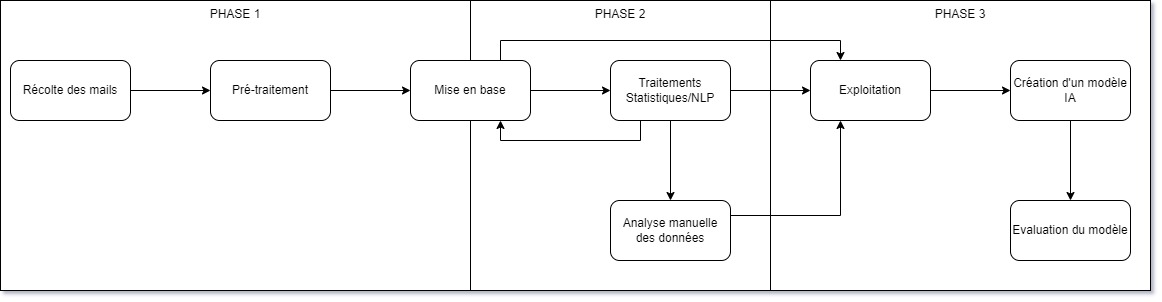
\includegraphics[width=\linewidth]{img/SchemaGeneral}
	\caption{Schéma des grandes étapes}
	\label{fig:SchemaGeneral}
\end{figure}

\subsection*{Mise en place de l'infrastructure opérationnelle}
	L'architecture opérationnelle s'appuie sur des conteneurs docker.
	Plusieurs types de base de données sont mises en œuvre profiter des avantages de chacune.
	Les conteneurs peuvent être gérés à l'aide du fichier \emph{Makefile} via les commandes suivantes :
	\begin{itemize}
		\item \emph{make docker\_start} : pour créer ou démarrer l'infrastructure
		\item \emph{make docker\_stop} : pour arrêter les conteneurs
		\item \emph{make docker\_prune} : pour nettoyer l'infrastructure
	\end{itemize}

	La figure~\ref{fig:Docker} montre l'organisation de cette architecture ainsi que les documents nécessaires pour son montage.
	\begin{figure}[H]
		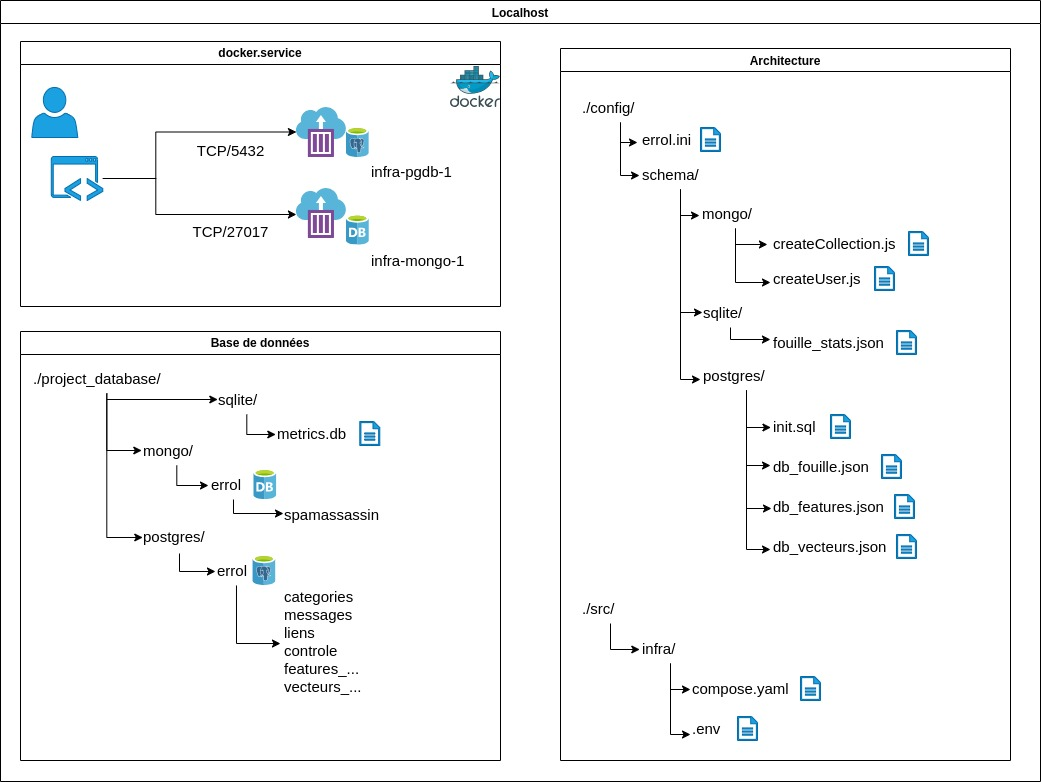
\includegraphics[width=\linewidth]{img/SchemaDocker}
		\caption{Schéma de l'architecture Docker}
		\label{fig:Docker}
	\end{figure}

	Les différentes tables et collections sont créées dynamiquement au cours des étapes du projet.

	\subsubsection*{Choix technologiques}
		\paragraph{Socle des services} 
			\subparagraph{Conteneurs}
				La conteneurisation des services permet d'effectuer facilement une séparation entre les processus.
				Les ressources empruntées à la machine hôte sont réduites au strict besoin de l'application.
				Une fois le moteur installé les différentes applications ou services peuvent être déployé rapidement.
				Chaque application embarque dans son conteneur toutes ses dépendances.
				Par définition les conteneurs sont volatils, des configurations complémentaires doivent être mises en place pour permettre la persistence des informations des bases de données.
				Solution retenue. \\
				Le moteur \emph{Docker} a été retenu, car il est simple d'utilisation, bien documenté et disponible sur plusieurs systèmes d'exploitation.
				Il est possible d'utiliser la capacité \emph{compose} de Docker pour déployer, démarrer ou arrêter plusieurs instances de manière coordonnée.

			\subparagraph{systemd}
				Une solution susceptible de fonctionner aurait été d'installer directement sur ma machine les différents services requis.
				Cela étant, un long processus d'installation puis de désinstallation aurait été nécessaire, avec le risque d'omettre des composants.
				De plus l'ajout de service directement sur la machine hôte comporte toujours des risques d'isolation des processus.
				Solution non retenue.

			\subparagraph{Machine virtuelle}
				L'installation des couches applicatives aurait pu être réalisé sur des machines virtuelles pour garantir une bonne isolation.
				Cela aurait également permit de simuler une infrastructure lourde avec plusieurs serveurs.
				Cependant, mon PC n'est pas en mesure de supporter l’exécution de plusieurs machines virtuelles en parallèle.
				Solution non retenue.

		\paragraph{Base NoSQL}
				Les bases de données NoSQL orientés documents sont plus performantes pour le stockage et l'accès à des ressources textuelles.
				Deux moteurs ont été testés :
			\subparagraph{MongoDB}
				Moteur de base données flexible et raisonnable en utilisation de ressource.
				Le langage des requêtes est simple à prendre en main.
				L'utilisation avec Python est facilitée par le \emph{Python developer path} disponible sur le site de l'éditeur.
				Solution retenue.

			\subparagraph{ElasticSearch}
				Moteur puissant de base de données qui intègre un moteur Lucène pour la recherche de document par mot clé.
				L'interface graphique associée (Kibana) est agréable et facile à prendre en main.
				Néanmoins, ce moteur est très gourmand en ressource.
				Une fois l'index (schéma) créé, il est très compliqué de le modifier.
				Solution rejetée.

		\paragraph{Base SQL}
			Les bases de données SQL sont plus performante quand il s'agit de traiter des informations transactionnelles.
			Elles offrent également plus de garantie de sécurité des données que les bases de données NoSQL\@.
			Elles permettent aussi de faire plus facilement et rapidement des requêtes complexes avec jointure et agrégation.
			Pour ces raisons, ce type de moteur sera utilisé pour stocker les informations numériques générées à partir des textes.
			\subparagraph{SQLite}
				Moteur de base de données SQL intégré avec Python.
				Les informations sont stockées dans un fichier défini.
				Cette base de données ne nécessite pas d'installer un service supplémentaire.
				Cette solution est généralement utilisée en phase de test.
				L'utilisation de cette solution pour stocker les données numériques des documents aurait été susceptible de générer des fichiers trop lourds et trop difficile à lier entre eux.
				Cependant, cette solution a été utilisée pour stocker les données générées lors de la phase de récolte (nombre de mails, nombre de mots uniques\ldots).
				Solution retenue

			\subparagraph{Postgres SQL}
				Moteur de base de données SQL solide et robuste.
				Elle permet également une gestion des utilisateurs ayant accès aux informations.
				L'intégration avec python est simple.
				Les données sont accessibles et peut être liées facilement.
				La taille des fichiers est gérée directement par le moteur.
				Solution retenue.